% vim: tw=80 noai
\documentclass[normaltoc,capchap,capsec,times]{abnt}
\usepackage[utf8]{inputenc}
\usepackage[T1]{fontenc}
\usepackage[brazil]{babel}
\usepackage[alf]{abntcite}
\usepackage[ordem=alf]{tabela-simbolos}
\usepackage{url}
\usepackage{graphicx}
\usepackage{listings}
\usepackage{verbatim}
\usepackage{subfigure}
\usepackage{multicol}
\usepackage{framed}
\usepackage{multirow}
\usepackage{longtable}
\usepackage{graphicx}
\usepackage[normalem]{ulem}
\usepackage{float}
\useunder{\uline}{\ul}{}
% O comando abaixo define o diretorio onde devem ser colocadas as imagens.
% Neste caso o diretorio é ./imagens/
\graphicspath{ {./imagens/} }
\def\lstlistingname{Listagem}

%%%%%%%%%%%%%%%%%%%%%%%%%%%%%%%%%%%%%%%%%%%%%%%%%%%%
% Dados do Trabalho
%%%%%%%%%%%%%%%%%%%%%%%%%%%%%%%%%%%%%%%%%%%%%%%%%%%%

\newcommand{\meunome}{José Lucas dos Santos Borges, Luiz Felipe Rosário}
\newcommand{\meutitulo}{Relações quantitativas dos indicadores sociais de pobreza e os índices de concentração de renda}
\newcommand{\meusubtitulo}{Um caso de aplicação da análise de regressão linear múltipla de dados dos Estados brasileiros}
\newcommand{\meuano}{2016}
\newcommand{\meuorientador}{\prof\ Carlos Khoury}

%%%%%%%%%%%%%%%%%%%%%%%%%%%%%%%%%%%%%%%%%%%%%%%%%%%%

%% O comando \obs aqui definido permite que o autor faca anotacoes no
%% trabalho que aparecem no PDF gerado. Para ativar o comando, descomente
%% a primeira linha e comente a segunda.
%% Exemplo de uso: \obs{Preciso melhorar este parágrafo...}

%\newcommand{\obs}[1]{\underline{\textbf{OBSERVAÇÃO}}: \emph{#1}}
\newcommand{\obs}[1]{}

\def\ordfem{\mbox{\raise .35em \hbox{\underline{\scriptsize a}\ }}}
\def\ordmasc{\mbox{\raise .35em \hbox{\underline{\scriptsize o}\ }}}
\def\profa{Prof\ordfem.}

%%%%%%%%%%%%%%%%%%%%%%%%%%%%%%%%%%%%%%%%%%%%%%%%%%%%

\begin{document}

% Capa com Brasão

\begin{titlepage}
   \begin{center}
    	%logotipo
               
\includegraphics[scale=0.3]{brasao_ufba} \\
	%\vspace{0.7in}
              \centering{ 
	      \bf{
	      \LARGE{
		\uppercase{UNIVERSIDADE FEDERAL DA BAHIA} \\
 	      }
	      \Large {
                   	\uppercase{FACULDADE DE ADMINISTRAÇÃO} \\
	      }
                   
              } }
   \end{center}
   \vfill
   \begin{center}
       \bf{
       \large{\uppercase{\meunome}  \\  }
       }
   \end{center}
   \vspace{0.2in}
   \begin{center}
       \bf{
      	 \LARGE{ \uppercase{\meutitulo} } \\
      	 \Large{ \uppercase{\meusubtitulo} }
         \obs{\\ \Large{Esta versão da monografia contém comentários do autor.
          Para removê-los, redefina o comando LaTeX \texttt{obs}.}}
       }
   \end{center}

   \vfill
   \hspace{\stretch{1}}
   \vfill
   \begin{center}
      \normalsize{
          Salvador \\
          \meuano
       }
   \end{center}

\end{titlepage}

%comando abaixo cria uma capa redundante, mas como a capa com brasão foi 
% feita 'manualmente', não faz sentido usar este comando:
%\capa



%% As listas a seguir sao opcionais:
%\listadetabelas
%\listadesiglas
%\listadesimbolos

\sumario

% O conteudo do trabalho esta' nos seguintes arquivos:
\chapter{Resumo}
\label{cap:resumo}
O artigo versa sobre a relação entre a taxa de mortalidade infantil e a taxa de cobertura de coleta de lixo juntamente com o índice de cobertura de esgotamento sanitário utilizando
dados de todas as capitais brasileiras no período de 2011. Este trabalho é importante por debater as condições de vida de milhões de brasileiros e apresentar algumas considerações sobre a
questão. Neste trabalho realizou-se uma regressão linear múltipla e foram feitos alguns testes para analisar a validade do modelo.

\textbf{Palavras-chave:} mortalidade infantil, desigualdade, saneamento, coleta de lixo, regressão linear.

\chapter{Introdução}
A mortalidade infantil é um problema social que ocorre em escala global e a redução
dela faz parte das Metas do Desenvolvimento do Milênio, compromisso assumido pelos países
integrantes da Organização das Nações Unidas (ONU), do qual o Brasil é signatário.

A taxa de mortalidade infantil consiste na relação entre o óbito de crianças no primeiro ano
de vida e a quantidade de nascidos vivos do mesmo período. Para facilidade de comparação entre
os diferentes países ou regiões do globo esta taxa é normalmente expressa em número de óbitos a
cada mil nascidos vivos.

No Brasil tem sido observado um declínio nesta taxa, como pode-se observar no gráfico a seguir:

\begin{center}
\begin{figure}[h]
  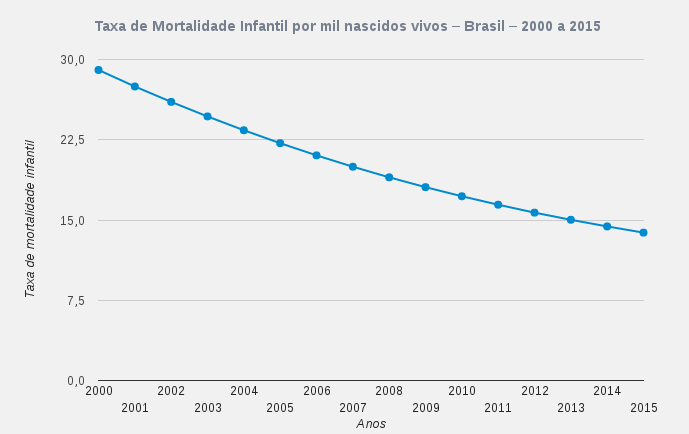
\includegraphics[width=\linewidth]{mortalidade_infantil.png}
\end{figure}
Fonte: \cite{ibgeMortalidade}
\end{center}

Apesar da significativa redução através dos anos, o Brasil ainda precisa melhorar
muito em relação aos países de primeiro mundo. A taxa de mortalidade atual (13,82/1000 nascidos vivos)
é cerca de três a seis vezes maior que a de países desenvolvidos, como Japão, Canadá e Alemanha que
apresentam taxa de 3 a 10/1000 nascidos vivos.

Numa situação ideal, esperaria-se que nenhuma criança morresse no primeiro ano de vida; nas situações
reais, é impossível reduzir a taxa de mortalidade infantil a zero, pois algumas crianças nascem com doenças
tão graves que a atual tecnologia médica disponível ainda não pode salvar suas vidas (ex: anencefalia).

Entretanto, a maioria das mortes precoces podem ser evitadas com o fácil e rápido acesso a serviços qualificados de saúde
e com a prevenção de doenças conhecidas. Além disso, fatores externos também
contribuem para a mudança desta taxa, como acesso ao  saneamento básico, taxa de fecundidade,
segurança alimentar e nutricional, grau de instrução das mulheres, avanço das tecnologias médicas,
em especial a imunização e terapia de reidratação oral, prevalência do aleitamento materno,
entre outros \cite{lansky2009mortalidade}, \cite{frias2008politicas}.

Para entender melhor a dinâmica da taxa de mortalidade infantil, estudar como cada um destes elementos
afeta a mesma torna-se uma necessidade.

A associação entre saneamento e saúde já foi objeto de inúmeros estudos \cite{libanio2005dimensao},
\cite{teixeira2011analise}, \cite{costa2002indicadores} e é consenso a afirmação de que o saneamento
básico afeta diretamente na qualidade de vida e mortalidade da população. Isso se explica pelas doenças
que são transmitidas em decorrência deste fato que afeta principalmente crianças e idosos
\cite{libanio2005dimensao}.

No âmbito do saneamento, dois fatores se destacam: A cobertura por esgotamento sanitário e a cobertura
por serviços de coleta de lixo. \cite{teixeira2011analise} diz que a baixa cobertura por esgotamento sanitário
nos estados brasileiros contribui para a mortalidade infantil no país. \cite{libanio2005dimensao} constata que a condição de vida das
populações é retratada pela abrangência dos serviços de água e esgoto e lixo.

Devido às evidências apresentadas, escolhemos fazer um estudo de regressão linear múltipla utilizando a
taxa de mortalidade infantil como variável dependente, e como variáveis independentes utilizamos a proporção
da população servida por esgotamento sanitário (dado em \%) e a proporção da população servida por coleta de
lixo (dado em \%).

Os dados utilizados foram retirados do site do IDB \cite{idb}, plataforma oficial do Ministério da Saúde para
assuntos relacionados.

Foram utilizados dois softwares para o processamento de dados estatísticos: Excel 2015 e o software R
através de sua plataforma web \cite{wessa}. O seguinte trabalho está estruturado da seguinte forma: seção 2.
Desenvolvimento da Regressão Linear. seção 3. Validação do modelo proposto, seção 4. Conclusão e seção 5
Referências Bibliográficas.

\chapter{Desenvolvimento}
\label{ref:desenvolvimento}


\chapter{Validação}



\chapter{Conclusão}
\label{cap:conclusao}



\bibliography{trabalho}

\end{document}
